\chapter{Localité des opérations}
	Ce chapitre traite de la gestion de la localité des opérations. Une
	opération est dite locale si elle n'affecte qu'une sous-région de l'image.

	Il est rapidement apparu que la gestion de ces opérations par l'algorithme
	de rasterisation présenté à la section précédente était loin d'être optimale,
	et ne permettait pas d'atteindre les objectifs d'interactivité du logiciel.

	Pour comprendre le problème, il faut d'abord comprendre comment fonctionne le
	logiciel de peinture. 
	\section{Le logiciel de peinture}
		Le logiciel de peinture possède trois outils principaux : La peinture,
		l'undo/redo, et une fenêtre de visualisation.
		\subsection{Background}
			Le logiciel présente à l'utilisateur une zone de dessin constituée d'un
			rectangle blanc qui représente la feuille sur laquelle dessiner. 
			Pour ce faire, nous utilisons une Frame unie et transparente comme source
			de l'hlImage, à laquelle nous ajoutons une opération de dessin d'un
			rectangle blanc. 
		\subsection{Peinture}
			La peinture se fait par la superposition de primitives appelées \emph{brushes}
			positionnées
			à intervalles réguliers sur le chemin tracé par l'utilisateur via la
			souris ou la tablette graphique. Les opérations de dessin de primitives 
			sont regroupées en traits, qui correspondent à une pression 
			continue sur le dessin. 

			La primitive utilisée pour la peinture est le cercle avec dégradé. Celui-ci
			est défini par deux rayons: Le rayon interne dans lequel le cercle est opaque,
			et le rayon externe, auquel se termine le cercle. Entre les deux un dégradé
			transparent. L'utilisateur peut aussi régler 
			l'opacité et la couleur de la primitive.

			Toutes les opérations sont ajoutées dans une seule hlImage, dont l'état
			est sauvegardé à chaque fin de trait.
		\begin{figure}[ht]
			\centering
			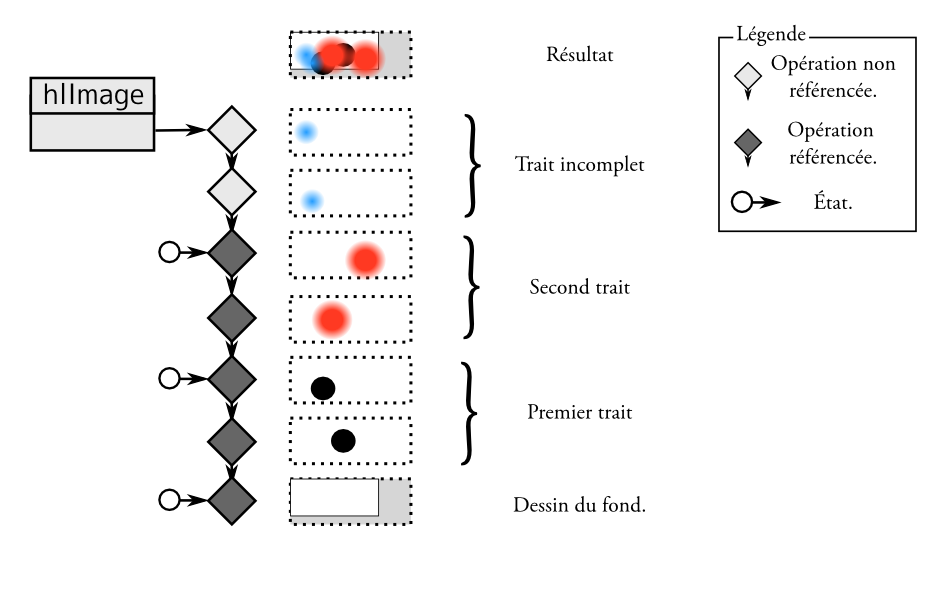
\includegraphics[width=\textwidth]{images/draw} 
			\caption{Fonctionnement de la peinture}
			\label{fig:draw}
		\end{figure}

			Ce mécanisme est résumé au schéma~\ref{fig:draw}, page~\pageref{fig:draw}.
			
		\subsection{Undo/Redo}
			L'undo redo fonctionne de la manière décrite au chapitre précédent.
			Une pile maintient une liste des états de chaque traits, permettant de défaire
			et refaire les opérations. 

			Comme indiqué au chapitre précédent, la consommation de mémoire est de
			l'ordre du nombre d'états. Comme il n'y a pas de mécanisme permettant de
			réguler les caches de manière globale, nous limitons le nombre d'états --- et donc d'undos --- disponibles
			à 16.
		\subsection{Visualisation}
			L'utilisateur visualise son dessin en temps réel via une fenêtre de visualisation.
			Celle-ci est décrite par sa taille en pixels, sa position sur le dessin, ainsi
			que son niveau d'échelle. 
			
			À chaque rafraîchissement (entre 30 et 60 fois par secondes), les tiles correspondant
			à la région sont identifiés, rasterisés, et copiés dans le buffer correspondant à la région
			afin d'être visualisés. 

			Les rafraîchissement se font indépendemment de l'ajout d'opérations. Un nombre quelconque
			d'opération peut donc avoir été ajouté entre deux rasterisations de l'image.

			L'utilisateur peut modifier la région de visualisation de trois manières différentes :

			\begin{itemize}
				\item Déplacer la région.
				\item Redimensionner la région.
				\item Changer l'échelle de visualisation.
			\end{itemize}

			Alors que déplacer et redimensionner la région ne demande que de recalculer les quelques tiles de la nouvelle
			bordure, changer l'échelle demande de recalculer l'entièreté de la région de visualisation. On peut
			donc s'attendre à ce que le déplacement et le redimensionnement de la région de visualisation soient 
			beaucoup plus rapides que le changement d'échelle.

	\section{Problématique}
		L'algorithme de rasterisation présenté jusqu'ici n'a aucune notion de localité d'opérations. Quelque soit le tile
		que nous voulons rasteriser, l'algorithme va appeler chacune des opérations. Si ces opérations ne s'appliquent pas
		au tile, celles-ci ne vont pas le modifier et vont donc s'exécuter très rapidement. Cependant, dans le cas de la 
		peinture, chaque tile n'est en réalité affecté que par un très petit pourcentage des opérations, et le nombre
		d'appel à ces opérations inutiles va en pratique ralentir de manière substantielle la rasterisation.

		Ce cas est particulièrement problématique lors du déplacement de la région de visualisation. Après avoir fait
		un large nombre de traits de peinture dans la région courante, l'utilisateur décide de déplacer la région de
		visualisation. De nouveaux tiles doivent donc être affichés. Pour ce faire l'algorithme de rasterisation va 
		examiner toutes les opérations des traits que l'utilisateur vient de dessiner, alors qu'aucun de ces traits n'affectent
		ces nouveaux tiles. 

		Il faut donc permettre à l'algorithme de rasterisation de pouvoir éviter d'examiner toute opération qui n'affecte
		pas les tiles. Au lieu d'avoir un algorithme de rasterisation en $O(n)$ ou $n$ est le nombre d'opérations
		ajoutées depuis le dernier rendu, nous aimerions avoir pour $n$ le nombre d'opérations ajoutées depuis le dernier
		rendu \emph{qui affectent le tile}.

		Il n'a pas été possible durant ce mémoire de trouver une réponse définitive à ce problème. Nous allons donc 
		passer en revue les différentes options qui ont été considérées, ainsi que leur efficacité. L'analyse de leur
		efficacité nous permet d'avoir une bonne idée de la direction à prendre pour la poursuite des recherches d'une
		solution à ce problème.

		Deux approches ont été testées: Les opérations vectorisées et les bounding operations. 	


	\section{Bounding Boxes}
\newcommand{\BB}{\emph{BB}~}
		Une première étape est d'ajouter à toutes les opérations de dessin une \emph{Bounding Box} --- \BB en abrégé.
		Celle-ci représente
		Une région rectangulaire, alignée aux axes de l'image, comprenant les tiles affectés par l'opération. Avant de rasteriser une opération 
		sur un tile, la \BB est examinée pour voir si le tile est affecté. s'il ne l'est pas, on peut éviter 
		de faire appel à la fonction de l'opération qui aurait de toute manière implémenté un tel mécanisme 
		de manière interne.

		Un autre intérêt d'un tel système est que la \BB est générée à la création de l'opération, et non à
		chaque appel de l'opération, ce qui améliore encore les performances.
		
		Pour réaliser cela, chaque classe d'opération doit donc être capable de générer de telles \BB.

		Si les \BB améliorent nettement les performances, elles n'améliorent pas la complexité
		temporelle de la rasterisation. Elles constituent cependant une base solide pour les deux solutions suivantes. 

	\section{Opérations vectorisées}
		\begin{figure}[ht]
			\centering
			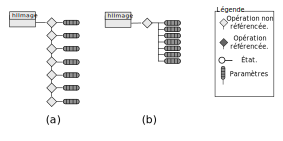
\includegraphics[width=\textwidth]{images/vector} 
			\caption{(a) Opérations normales, (b) Opérations vectorisées}
			\label{fig:vector}
		\end{figure}
		Vectoriser les opérations consiste à regrouper des opérations du même type en une seule opération qui contient
		un vecteur de paramètres représentant l'ensemble des paramètres. La \BB de l'opération
		vectorisée englobant les \BB des opérations qui la composent. Ceci est représenté au 
		schéma~\ref{fig:vector}, page~\pageref{fig:vector}
		Les opérations vectorielles ont plusieurs intérêts:
		\begin{itemize}
			\item La structure hlOperation est mise en commun, permettant d'économiser la mémoire.
			\item Si un paramètre des opérations est constant dans le vecteur, celui-ci peut être mis en commun,
			ce qui économise de la mémoire. Ce cas de figure se présente régulièrement en peinture; les traits étant principalement
			composés de \emph{brushes} de même couleur et de même diamètre.
			\item Un test sur la Bounding box de l'opération vectorielle permet d'éviter le test de l'intégralité
			des opérations internes.
		\end{itemize}
		Mais ne sont pas sans limites:
		\begin{itemize}
			\item Il n'est pas possible de vectoriser des opérations de type différent. Ce système ne fonctionnerait
			donc pas pour un pinceau qui peindrait une alternance de cercles et de carrés.
			\item Il n'est pas possible de placer un état au milieu d'opérations vectorisées.
			\item L'algorithme de rasterisation doit être lourdement modifié pour pouvoir supporter ce type d'opérations.
			\item Les opérations vectorisées ne peuvent être modifiées avec l'API classique.
		\end{itemize}
				\begin{table*}
					\centering
					\begin{tabular*}{0.7\textwidth}{@{\extracolsep{\fill}} | c | c |}
					\hline
					Dessin & Nombre moyen d'opérations par trait \\
					\hline
					A	& 105.4 \\
					B	& 199.8 \\
					C	& 117.8 \\
					D	& 149.1 \\
					E	& 117.2 \\
					\hline
					\end{tabular*}
					\caption{Nombre moyen d'opérations par trait sur les dessins de tests (voir figure~\ref{fig:testdrawings}, 
					page~\pageref{fig:testdrawings}) }
					\label{strokelength}
				\end{table*}
		Les performances des opérations vectorisées seront donc contraintes par le nombre d'opérations du même type que
		l'on trouve entre chaque état. Pour l'application de peinture développée, les opérations sont toujours du même
		type, et un trait faisant en moyenne une centaine d'opérations (voir tableau~\ref{strokelength}, page~\pageref{strokelength}), 
		le nombre de tests de bounding box à réaliser en 
		dehors des traits est divisé par 100. Le nombre de tests à réaliser sur les traits, augmente en contrepartie d'un
		pourcent à cause de la \BB supplémentaire.

		Nous n'atteignons donc pas notre objectif de réduction de complexité, mais les opérations vectorisées permettent
		de réduire de deux ordres de grandeur le coût de la localité des opérations.

		\subsection{Impact sur l'API}
		Étant donné les limitations des opérations vectorisées, nous sommes obligés de donner à l'utilisateur un
		certain contrôle sur celles-ci. Nous proposons donc une fonction supplémentaire :
			\paragraph{\lstinline$void hlOpVectorise(hlOperation *op)$}
			\begin{description}
				\item[pre]: op est une opération qui n'est pas encore insérée dans la pile.
				\item[post]: op est une opération vectorisée. Toute opération non vectorisée du même
				type qu'op insérée sur la pile au dessus de op sera vectorisée dans op, jusqu'à ce
				que op soit sauvegardée dans un état.
			\end{description}
		Ainsi, l'utilisateur n'a qu'à utiliser cette fonction sur la première opération de chaque trait pour pouvoir
		vectoriser les traits. 
		\subsection{Évaluation des performances}
		À part un gain de mémoire au niveau de la description du document, qui reste négligeable par rapport au poids pris
		par les caches, les performances démontrées par les opérations vectorisés sont quasiment identiques à un cas particulier
		des Bounding Opérations, solution plus prometteuse présentée à la section suivante.

		Nous nous référerons donc à la section \emph{Évaluation des performances / Tailles des \emph{BO}} 
		pour un aperçu des performances des opérations vectorisées.  

	\section{Bounding Opérations}
\newcommand{\BO}{\emph{BO}~}
		\begin{figure}[ht]
			\centering
			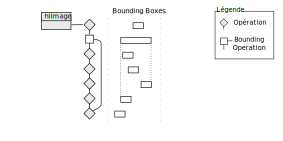
\includegraphics[width=\textwidth]{images/bo} 
			\caption{Une Bounding Opération}
			\label{fig:bo}
		\end{figure}
		Les \emph{Bounding Opérations} -- \BO en abrégé --- ne sont pas des opérations au sens original du terme puisque si utilisées
		correctement, elles n'effectuent aucune modification de l'image. Cependant elles s'utilisent et s'insèrent
		dans la pile comme des opérations classiques  appartenant à une nouvelle catégorie.  Leur but est d'offrir une \BB englobant
		plusieurs opérations, de la même manière que les opérations vectorisées, mais de manière plus flexible et facile à implémenter:

		\subsection{Principes d'une \BO}
		
		Les \BO contiennent une \BB et une référence vers une opération antérieure.
		La rasterisation des \emph{Bounding Opérations} fonctionne de la manière suivante:
		\begin{itemize}
			\item Rasteriser un tile à l'intérieur de la \BB consiste à rasteriser l'opération précédente.
			\item Rasteriser un tile à l'extérieur de la \BB consiste à rasteriser l'opération antérieure référencée.
		\end{itemize}

		En créant une \BO dont la \BB englobe les \BB d'une suite
		d'opérations qui la précèdent, et en faisant pointer la \BO sur une opération précédant 
		cette suite, on permet à l'algorithme de rasterisation de contourner la suite d'opérations.
		
		Ce principe est représenté au schéma~\ref{fig:bo}, page~\pageref{fig:bo}

		Les \BO ne modifiant pas l'apparence de l'image, on peut les placer où l'on veut dans la pile. Ces 
		opérations peuvent donc "enjamber" des états, permettant des groupements qui ne sont pas possibles avec les opérations
		vectorisées.

		\begin{figure}[ht]
			\centering
			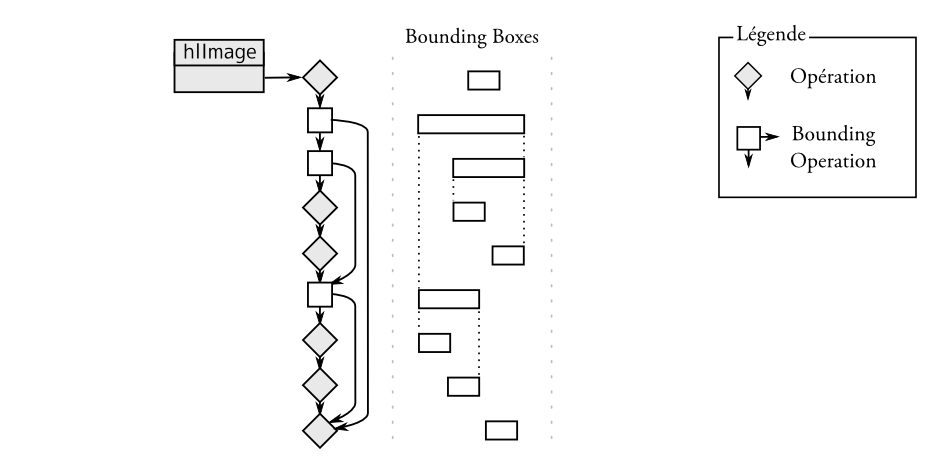
\includegraphics[width=\textwidth]{images/bo2} 
			\caption{Une Bounding Opération Hierarchy}
			\label{fig:bo2}
		\end{figure}

		Là où les \BO deviennent très intéressantes c'est qu'on peut les emboîter les unes dans les
		autres de manière récursive, et ainsi offrir une structure semblable à une \emph{Bounding Volume Hierarchy}\cite{shirley} 
		--- \emph{BVH} en abrégé --- ou à des \emph{KD-Trees}\cite{shirley}. On appelle \emph{Bounding Opération Hierarchy} --- \emph{BOH}
		en abrégé --- L'implémentation par des \BO de ce type de structures. Lorsque les \BO ne s'imbriquent pas, on parle alors de \emph{Bounding Object Sequence},
		--- \emph{BOS} en abrégé. Un exemple de \emph{BOH} est représenté au schéma~\ref{fig:bo2}, page~\pageref{fig:bo2} 

		\begin{figure}[ht]
			\centering
			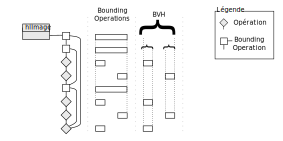
\includegraphics[width=\textwidth]{images/bo3} 
			\caption{Cas critique pour les \emph{BOH}}
			\label{fig:bo3}
		\end{figure}
		Il y a cependant une grande différence entre les \emph{BVH}, et les \emph{BOH}; là où un \emph{Bounding Volume}
		peut contenir n'importe quel ensemble
		d'objets dans la scène, une \BO ne peut contenir que des opérations qui sont adjacentes dans la pile. Il
		est très simple de construire un exemple ou les \emph{BVH} excellent et les \emph{BOH} ne font qu'empirer
		les choses, comme sur le schéma~\ref{fig:bo3}, page~\pageref{fig:bo3}. Heureusement de tels cas arrivent peu 
		en pratique, puisque les outils de peinture tendent à grouper les opérations de manière adéquate.

		Il serait cependant possible d'approcher l'efficacité d'un \emph{BVH} en procédant à un réordonancement intelligent
		des opérations. 
		
		Une autre différence de taille est que les \emph{BVH} sont conçus pour organiser des scènes statiques,
		et non pour des scènes pouvant changer selon les états. Ces différences nous empêchent de reprendre 
		les algorithmes développés pour les \emph{BVH} et les \emph{KD-Trees}, 
		même si nous pouvons en reprendre les idées et les principes. 

		Une première tâche intéressante consiste à construire la \emph{BOH}. La littérature\cite{havran} sur les \emph{BVH}
		décrit deux types d'algorithmes:
		\begin{description}
			\item[Algorithmes Inline] Ces algorithmes construisent la \emph{BVH} au fur et à mesure
			que l'on ajoute des objets dans la scène --- des opérations dans l'image. Ces algorithmes 
			semblent donc particulièrement adaptés à la peinture puisqu'ils fonctionneront au fur et à mesure que l'utilisateur
			peint. Ces algorithmes 
			\item[Algorithmes Offline] Ces algorithmes construisent la \emph{BVH} à partir d'une 
			scène déjà construite --- d'un pile d'opération existante. Ces algorithmes ont l'avantage de pouvoir
			créer des hiérarchies optimales (selon différents critères). Le problème est qu'ils prennent un certain temps 
			à s'exécuter, ce qui n'est pas idéal pour un framework dédié à l'édition interactive. 
		\end{description}
		Seul des algorithmes inline ont pour l'instant été explorés et implémentés. Un algorithme crée des \emph{BOS} ,
		et l'autre des \emph{BOH}. 
		
		\subsection{Bounding Opération Sequence}
			Le premier algorithme testé et implémenté est un algorithme créant un \emph{BOS}
			
			\subsubsection{Placement des \BO dans la pile}
			Le placement des \BO dans la pile fonctionne de la manière suivante: Initialement, la \BO possède une \BB
			de taille nulle, et est dans l'état dit \emph{ouvert} Lorsque l'on insère cette \BO au dessus de la pile, 
			celle-ci prend pour comme opération de référence l'opération précédente. 

			Lorsque l'on insère une opération sur la pile, au dessus d'une \BO ouverte, la \BB de la \BO est étendue
			pour englober la \BB de la nouvelle opération. La \BB est ensuite repositionnée au dessus de la pile. 

			L'on peut continuer à insérer des opérations de cette manière jusqu'à ce que la \BO soit \emph{fermée},
			auquel cas elle se comporte comme une opération normale. 

			\subsubsection{Fermer les \emph{Bounding Opérations}}
			Ce premier algorithme va donc ajouter des \BO ouvertes, les fermer au moment opportun et puis directement 
			en rajouter une nouvelle ouverte. Il s'agit donc de savoir quand fermer les \BO.

			L'impact des performances des \BO peut se répartir en deux cas\footnote{cette discussion est équivalente à celles motivant les \emph{Bounding Area Heuristics} utilisées pour la construction de \emph{KD-Trees} ou \emph{BVH}\cite{havran}} :
			\begin{description}
				\item[Rendu d'un tile à l'extérieur de la \BO]: Dans ce cas, on doit effectuer un test de \BB de la \BO
				uniquement. Comme on aimerait diminuer le nombre de tests de \BB, on aimerait donc avoir un nombre minimal
				de \BO.
				\item[Rendu d'un tile à l'intérieur de la \BB]: Dans ce cas, on doit tester les \BB de toutes les 
				opérations à l'intérieur de la \BO, que celles ci influence le tile ou pas. On aimerait donc avoir le moins
				de Rendus à l'intérieur de \BO. Statistiquement, plus la surface de la \BB d'une \BO est petite, moins de
				tiles seront rendus à l'intérieur. On aimerait donc avec des \BO avec les \BB les plus petites possibles.
			\end{description}
			
			La fermeture des \BO doit donc satisfaire deux critères: avoir le moins de \BO, et avoir les \BO les plus petites. 
			Ces deux critères étant opposés, nous allons examiner leur importance en examinant différents schémas de fermeture
			dans la section \emph{analyse de performances}
			

		\subsection{Bounding Opération Hierarchy}
			Cet algorithme permet de créer une hiérarchie de \BO d'une profondeur fixe. Dans cet algorithme chaque niveau
			fonctionne exactement comme l'algorithme précédent en considérant les \BO des opérations d'en dessous comme
			des opérations classiques. Une première analyse d'efficacité se trouve à la section \emph{Analyse des performances}


		\subsection{Impact sur l'API}
			Les \BO ont un impact minimal sur l'API. Il suffit d'ajouter une opération de type \BO avec les paramètres
			appropriés pour que les mécanismes se mettent en place. Une fois en place les \BO n'influent quasiment pas
			sur les actions que l'on peut réaliser sur une hlImage. 

			Par contre, le fait que les \BO puissent être déplacées automatiquement par d'autres opérations perturbe
			l'accès aux opérations par indice. Pour résoudre ce problème, les \BO sont ignorées lors des accès par
			indice. 

			Si l'algorithme de rasterisation ne doit pas être grandement modifié, les algorithmes de modification
			de la pile doivent être revus pour préserver la cohérence des \emph{BOH}.

			\subsubsection{Forking}
			\begin{figure}[ht]
				\centering
				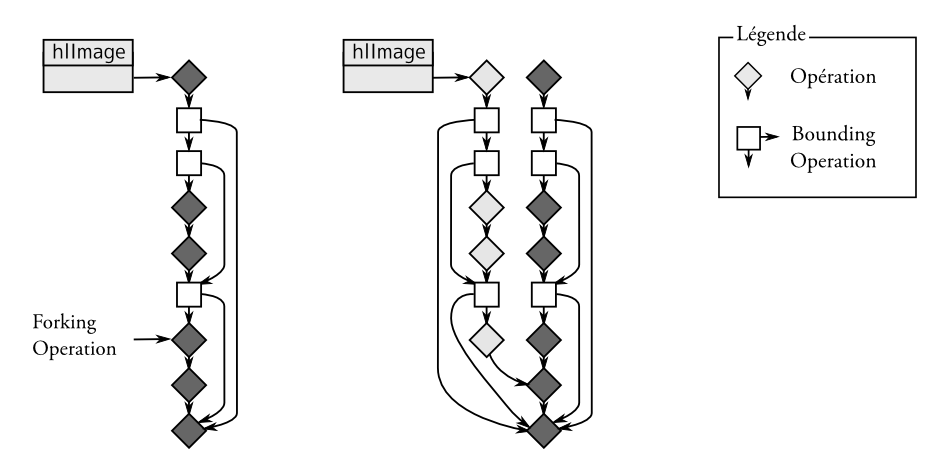
\includegraphics[width=\textwidth]{images/bo-forking} 
				\caption{Forker des \BO}
				\label{fig:bo-forking}
			\end{figure}
			L'opération de forking doit duplique également les \BO. Le schéma~\ref{fig:bo-forking}, page~\pageref{fig:bo-forking} montre une pile
			contenant des \BO avant et après forking. 

			La difficulté réside donc à réassocier les références correctement. 
			Ceci se fait en reprenant l'algorithme de forking en appliquant les modifications suivantes:
			\begin{itemize}
				\item Lorsque l'on duplique une \BO, son duplicata continue à pointer vers l'opération originale.
				On associe ensuite dans une Hashtable l'uid de l'opération pointée
				par la \BO à cette \BO. 
				\item Lorsque l'on duplique une opération (\BO comprises), on regarde si son uid est présente dans
				la Hashtable. Dans l'affirmative, la \BO correspondante pointe désormais sur cette opération, et
				l'uid est retiré de la Hashtable.
			\end{itemize}
			L'opération de forking garde donc toujours la même complexité temporelle, mais gagne une complexité spatiale
			de $O(n)$ où $n$ est la profondeur maximale de la \emph{BOH}, la profondeur des \emph{BOH} étant en $O(log(n))$, où $n$
			est le nombre total d'opérations dans la pile. 
			
			\subsubsection{Retrait d'opérations}
			\begin{figure}[ht]
				\centering
				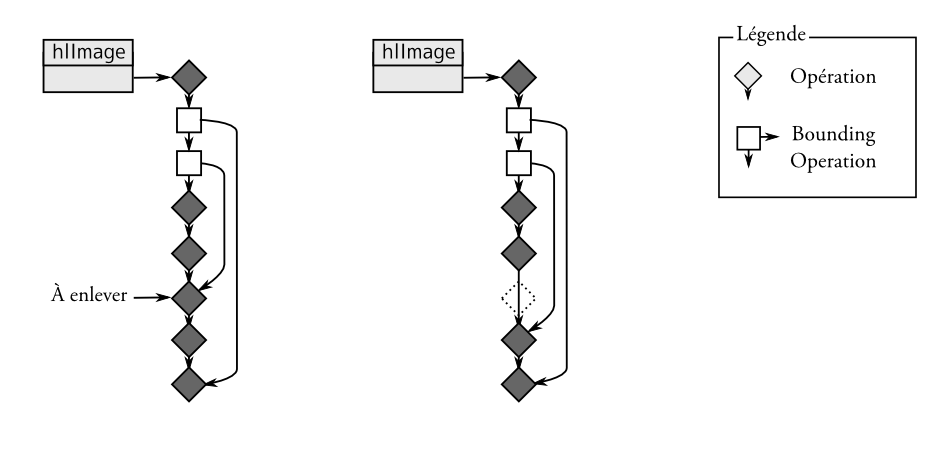
\includegraphics[width=\textwidth]{images/bo-supress} 
				\caption{Retirer une opération pointée par une \BO}
				\label{fig:bo-supress}
			\end{figure}
			Le retrait d'une opération dans la pile peut être problématique si un \BO pointe sur cette opération. Dans de
			tel cas, il faut détecter les \BO qui pointent et les faire pointer vers l'opération précédente à celle
			que l'on veut retirer. Si il n'y a pas de telle opération précédente, on met la référence à \emph{NULL} pour indiquer qu'il faut accéder directement à la source de l'image.
			Il faut également supprimer les \BO qui ne contiennent d'opération autre
			que des \BO.  Un exemple de retrait d'opération dans une pile contenant des \BO est représenté au 
			schéma~\ref{fig:bo-supress}, page~\pageref{fig:bo-supress}
			
			Ceci ne modifie pas la complexité temporelle, mais ajoute une complexité spatiale
			de $O(n)$ ou $n$ est le nombre de \BO pointant l'opération à retirer. Ce nombre est également borné par
			la profondeur de la \emph{BOH}, ce qui ramène cette complexité à $O(log(n))$ ou $n$ est le nombre d'opérations dans
			la pile jusqu'à l'opération à retirer. 

			\subsubsection{Insertion et Modification d'opérations}
			\begin{figure}[ht]
				\centering
				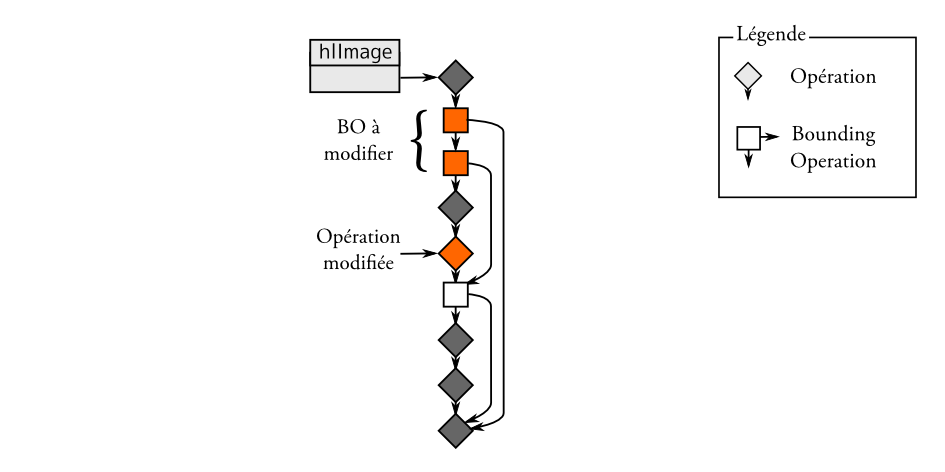
\includegraphics[width=\textwidth]{images/bo-modify} 
				\caption{Modifier une opération dans une pile contenant des \BO}
				\label{fig:bo-modify}
			\end{figure}
			Insérer ou modifier des opérations peut invalider les \BB des \BO qui englobent ces opérations. Il faut
			donc détecter ces \BO, et modifier leur \BB afin qu'elles contiennent la \BB de l'opération à insérer, ou la
			nouvelle \BB de l'opération modifiée, ce qui se fait en parcourant la pile jusqu'à l'emplacement d'insertion,
			ou jusqu'à l'opération à modifier de la manière suivante
			\begin{itemize}
				\item Lorsque l'on rencontre une \BO, on l'associe dans une Hashtable à l'opération pointée.
				\item Lorsque l'on rencontre une opération, on retire la \BO associée dans la Hashtable.
				\item Lorsque l'on arrive à l'emplacement voulu, ou à l'opération à modifier, la Hashtable
				contient la liste des \BO à modifier.
			\end{itemize}
			Cela ne modifie donc pas la complexité temporelle, mais ajoute une complexité spatiale, en $O(log(n))$ où $n$
			est le nombre d'opérations dans la pile.

		\subsection{Évaluation des performances}
			Pour évaluer les performances, nous avons enregistré les étapes de création de plusieurs dessins, chacun d'entre eux représentant
			un cas d'utilisation différent. Ces dessins de taille variable ont été réalisés sur une feuille de $4.8*10^{17}$ pixels. Nous avons 
			ensuite rejoué ces étapes (ajout d'opérations, rasterisation, zoom, dézoom, undo, redo,
			déplacement du viewport) en omettant les pauses afin de mesurer le temps total pris par le framework pour dessiner le dessin.
			
			Toutes les expériences ont été réalisées sur une machine disposant d'un processeur \emph{Intel Core Duo 2400} à deux cores cadencés
			à 1.66GHz, et disposant de 2Go de mémoire vive. 

			\begin{figure}[h]
				\centering
				\captionsetup[subfigure]{labelformat=empty}
				\subfloat[$(a)$~Dessin technique, 25Mpixels]{ 
\includegraphics[width=0.5\textwidth]{images/tests/test_a} }
				\subfloat[$(b)$~Hachures, $0.5$Gpixels]{ \label{fig:testb} 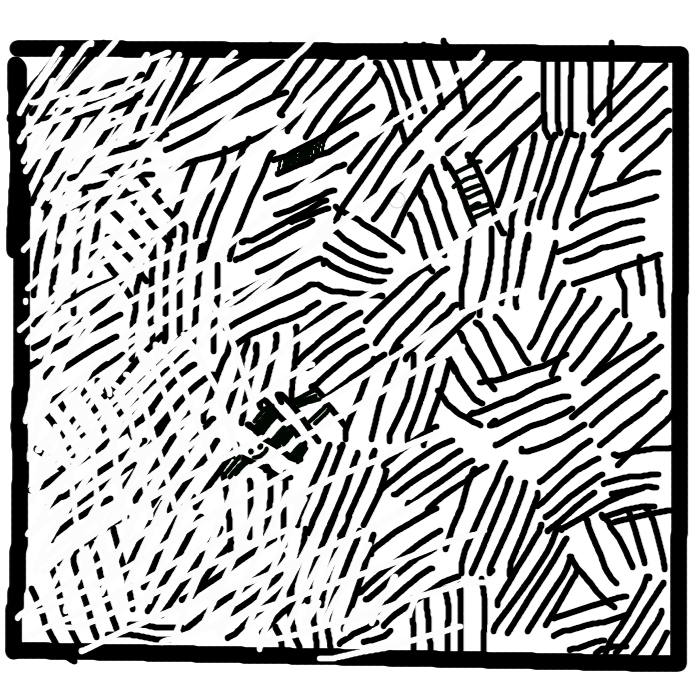
\includegraphics[width=0.5\textwidth]{images/tests/test_b} }
				\\
				\subfloat[$(c)$~Portrait, $25$Mpixels]{ \label{fig:testc} 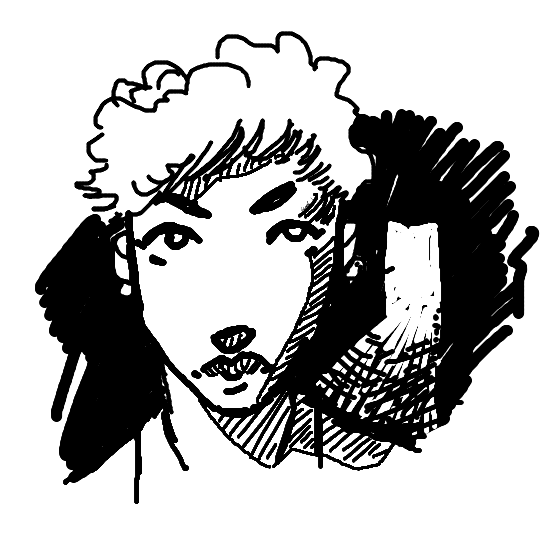
\includegraphics[width=0.5\textwidth]{images/tests/test_c} }
				\subfloat[$(e)$~Test divers, $0.5$Gpixels]{ \label{fig:teste} 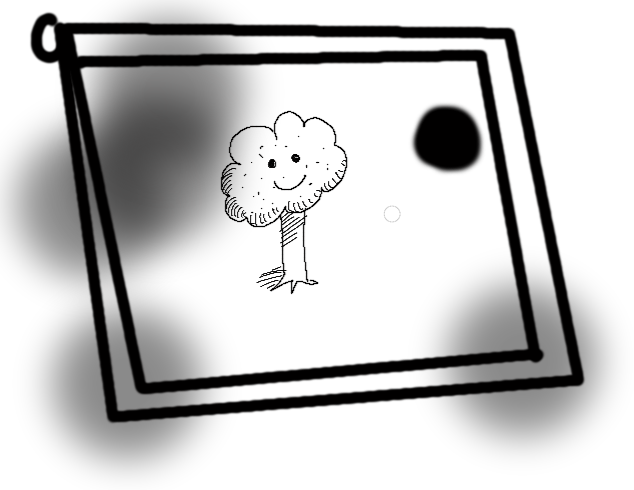
\includegraphics[width=0.5\textwidth]{images/tests/test_e} }
				\\
				\subfloat[$(d)$~Paysage avec petits détails, $2$Gpixels]{ \label{fig:testd} 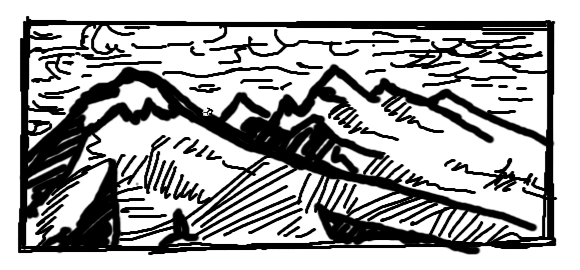
\includegraphics[width=\textwidth]{images/tests/test_d} }
				\caption{Dessins utilisés pour les tests de performances}
				\label{fig:testdrawings}
			\end{figure}

			Les cinq dessins sont présentés à la figure~\ref{fig:testdrawings}, page~\pageref{fig:testdrawings}. Chacun d'entre eux a été
			réalisé pour simuler un cas d'utilisation différent:
			\begin{description}
				\item[A] Ce dessin représente un dessin technique, composé essentiellement de lignes droites d'orientation similaires, ainsi
				que d'arcs de cercles. 
				\item[B] Ce dessin représente des hachures, qui peuvent constituer l'essentiel d'un dessin au trait.
				\item[C] Ce portrait est destiné à représenter un dessin complet qui comprend une variété de technique différentes : traits de contour,
				remplissages, hachures, ...
				\item[D] Ce paysage de grande taille contenant de très petits éléments simule l'utilisation du framework pour l'édition d'images
				gigapixel à des échelles fort différentes.
				\item[E] Ce dessin est constitué de différents éléments ayant posé problèmes lors des tests de performances, comme par exemple 
				des brushes et des traits de taille très différentes. 
			\end{description}
			Ces dessins sont en noir et blanc pour limiter le nombre d'opération nécessaires à leur réalisation. En effet les dessins ont été faits 
			suffisamment petits pour limiter le temps de calcul lors de l'évaluation des performances. Ces dessins ne sont donc pas totalement
			représentatifs de ce qui se fait en conditions réelles, mais devraient être suffisamment proche pour nous permettre de savoir quelle
			solutions gagneraient à être explorées plus en détail sur des données en provenance de tests utilisateurs.

			\subsubsection{Taille des \BO}
				Le premier test utilise une heuristique qui ferme la boite quand celle-ci contient un certain nombre d'opérations, ou
				quand un nouvel état est enregistré. À noter que cette heuristique correspond exactement au système d'opération vectorisées,
				qui produit des temps de calculs quasiment identiques. 

				\begin{table*}
					\tiny
					\begin{tabular*}{\textwidth}{@{\extracolsep{\fill}} | c || c | c | c | c | c | c | c | c | c | c |}
						\hline
						& \multicolumn{10}{c|}{Nombre maximal d'opérations par \BO} \\
						\hline
								&8		&  16		&  32		&  64		&  128		&  256		&  512		&  1024		&  2048		&  4092		 \\
						\hline
						\hline
						Dessin & \multicolumn{10}{c|}{Temps de calcul (sec)} \\
						\hline
						 A		& 249.67	&  117.81	&  72.01	&  52.00	&  39.13	&  34.32	&  32.87	&  32.84	&  32.99	&  32.83	 \\
						 B 		& 847.67	&  312.65	&  113.12	&  70.14	&  52.35	&  40.44	&  39.45	&  41.32	&  42.51	&  42.78	 \\
						 C		& 1283.64	&  550.17	&  354.88	&  154.36	&  138.46	&  163.26	&  104.11	&  94.40	&  108.18	&  146.60	 \\
						 D		& 1181.11	&  466.45	&  278.11	&  144.25	&  170.93	&  132.44	&  91.03	&  89.84	&  88.35	&  140.39	 \\
						 E		& 61.32		&  38.71	&  18.21	&  12.93	&  11.81	&  11.19	&  11.01	&  11.08	&  10.72	&  11.15	 \\
						\hline
					\end{tabular*}
					\caption{\label{boxdepth} Performances de la première heuristique de fermeture des \BO}
				\end{table*}
				\begin{figure}[h]
					\centering
					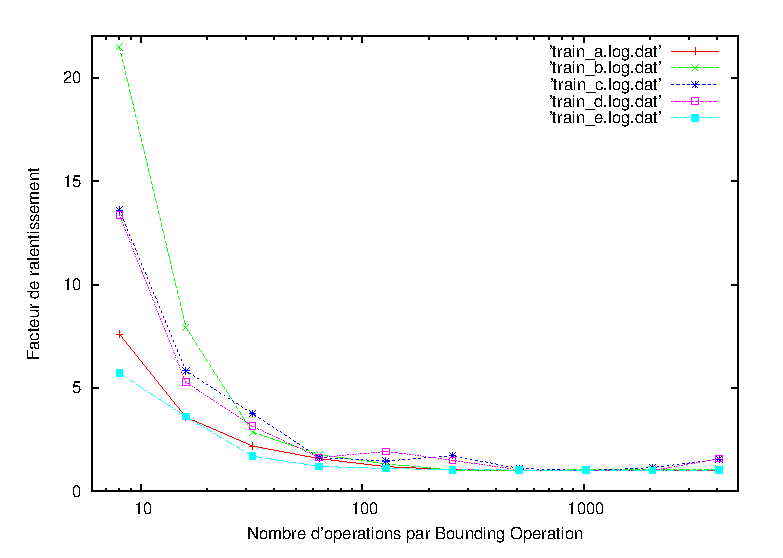
\includegraphics[width=\textwidth]{images/depthgraph.eps} 
					\caption{\label{fig:depthgraph}Peformances de la première heuristique normalisées par leur meilleur temps}
				\end{figure}
				
				Le tableau~\ref{boxdepth}, page~\pageref{boxdepth}, reprend les résultats des expériences pour différentes tailles de boites.
				Le graphe~\ref{fig:depthgraph}, page~\pageref{fig:depthgraph} reprend ces données en normalisant les durées d'exécution de chaque
				test sur la durée la plus rapide. 

				On peut y voir que les performances augmentent avec la taille des \BO pour ne jamais redescendre. On en déduit donc que 
				la taille de la boite importe beaucoup moins que leur nombre. Si les performances ne diminuent pas plus au delà d'un
				certain nombre d'opérations par \BO, c'est parce qu'à partir d'un certain point, les \BO sont toutes fermées par 
				l'enregistrement d'un nouvel état. 

			\subsubsection{Aire accumulée}
				Cette heuristique basée sur l'aire accumulée essaie d'établir un compromis entre la taille des \BO et le nombre d'opérations
				contenues dans celles-ci:

				A chaque fois que l'on insère une opération dans une \BO, on évalue l'augmentation de la surface de la \BB de celle-ci. 
				On normalise ensuite cette augmentation de surface par la taille de la \BB de l'opération ajoutée. Cette augmentation
				de surface est accumulée dans un compteur dans la \BO. Lorsque celle-ci dépasse un seuil, la \BO est fermée. 

				Cette heuristique favorise donc des \BO plus denses, ce qui l'on espère, permettra d'avoir une meilleure répartition des
				\BO.

				\begin{table*}
					\tiny
					\begin{tabular*}{\textwidth}{@{\extracolsep{\fill}} | c || c | c | c | c | c | c | c | c |}
						\hline
						& \multicolumn{8}{c|}{Aire maximale accumulée par \BO} \\
						\hline
								& 2		& 4		& 8		&  16		&  32		&  64		&  128		&  512		\\
						\hline
						\hline
						Dessin & \multicolumn{8}{c|}{Temps de calcul (sec)} \\
						\hline
						A		& 70.85		&  51.89	&  41.54	&  37.51	&  35.72	&  34.89	&  36.23	&  54.46	\\
						B		& 225.32	&  139.10	&  100.74	&  83.29	&  45.69	&  42.70	&  41.45	&  43.58	\\
						C		& 585.40	&  321.23	&  141.87	&  163.36	&  156.43	&  145.06	&  143.24	&  141.66	\\
						D		& 656.04	&  358.37	&  158.52	&  153.24	&  159.39	&  149.18	&  148.01	&  98.38	\\
						E		& 16.21		&  12.59	&  11.73	&  12.30	&  11.44	&  10.62	&  11.13	&  10.66	\\
						\hline
					\end{tabular*}
					\caption{\label{boxratio} Performances de la seconde heuristique}
				\end{table*}
				\begin{figure}[h]
					\centering
					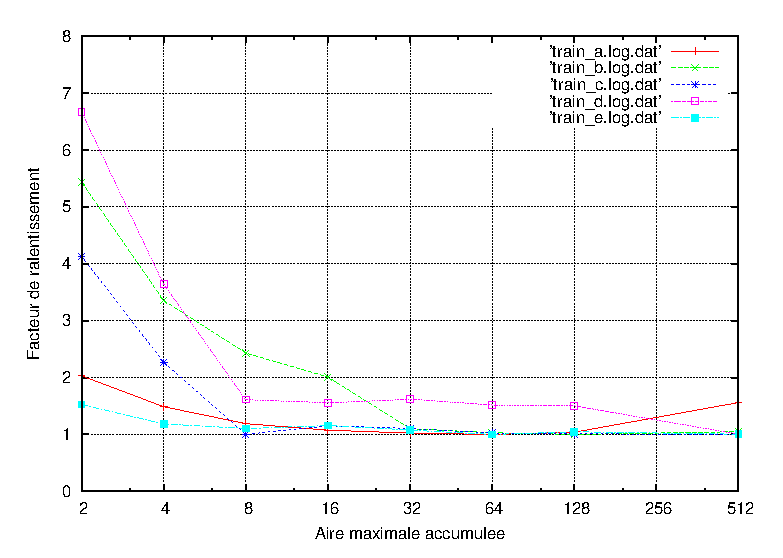
\includegraphics[width=\textwidth]{images/graph_ratio.eps} 
					\caption{\label{fig:ratiograph}Performances de la seconde heuristique normalisées par leur meilleur temps}
				\end{figure}
				Les résultats des expériences sont repris au tableau~\ref{boxratio}, page~\pageref{boxratio}. Celles-ci sont également
				reprises normalisées sur leur meilleur temps au graphe~\ref{fig:ratiograph}, page~\pageref{fig:ratiograph}.

				On constate tout d'abord que cette heuristique ne permet pas d'atteindre les temps atteints par la précédente. On constate
				ensuite que l'évolution des améliorations est moins régulière et reflète les différences de structure des différentes images. 
				Cette évolution irrégulière a pour conséquence qu'aucune valeur n'est optimale pour tous les tests, indiquant que la limite doit
				être modulée en fonction de l'utilisation du framework. 

				On constate également que cette heuristique fonctionne le moins bien pour les images \emph{A} et \emph{C}, qui contiennent
				beaucoup de diagonales.  Le problème de cette heuristique avec ces diagonales c'est que celles-ci sont particulièrement mal
				épousées par les \BB qui sont alignées aux axes. Dans ces cas l'aire est accumulée quadratiquement avec la longueur, et donc
				les boites sont clôturées trop tôt. Ceci génère un trop grand nombre de \BO, et comme le résultat de l'expérience précédente
				nous indique, les performances sont fortement affectées lorsque celles-ci sont trop nombreuses.

			\subsubsection{\emph{BOH}}
				Nous utilisons pour cette troisième heuristique une \emph{BOH} à deux niveaux. Les \BO du premier niveau se clôturent
				au delà d'un nombre fixe d'opérations, de la même manière que la première heuristique. Les \BO du second niveau ne sont
				quand à elles clôturées qu'à l'ajout d'un nouvel état. Cette heuristique permet donc d'évaluer les gains que l'on peut
				obtenir en rajoutant un second niveau. 
				\begin{table*}
					\tiny
					\begin{tabular*}{\textwidth}{@{\extracolsep{\fill}} | c || c | c | c | c | c | c | c | c | c | c |}
						\hline
						& \multicolumn{10}{c|}{Nombre maximal d'opérations par \BO} \\
						\hline
								&8		&  16		&  32		&  64		&  128		&  256		&  512		&  1024		&  2048		&  4092		 \\
						\hline
						\hline
						Dessin & \multicolumn{10}{c|}{Temps de calcul (sec)} \\
						\hline
						A		& 56.33		&  35.43	&  33.72	&  33.41	&  33.57	&  33.32	&  32.82	&  34.31	&  34.76	&  34.26	\\
						B		& 53.30		&  70.24	&  67.47	&  66.61	&  64.70	&  41.40	&  42.01	&  43.41	&  44.54	&  44.36	\\
						C 		& 107.27	&  144.32	&  141.42	&  94.17	&  91.31	&  123.96	&  142.79	&  141.63	&  142.71	&  148.53	\\
						D		& 144.20	&  88.20	&  86.48	&  115.26	&  140.11	&  147.81	&  141.73	&  101.48	&  88.51	&  108.78	\\
						E		& 17.88		&  17.06	&  16.89	&  16.67	&  16.32	&  16.59	&  16.51	&  16.59	&  16.88	&  16.28	\\
						\hline
					\end{tabular*}
					\caption{\label{boxdepth1}Performances de la troisième heuristique}
				\end{table*}
				\begin{figure}[h]
					\centering
					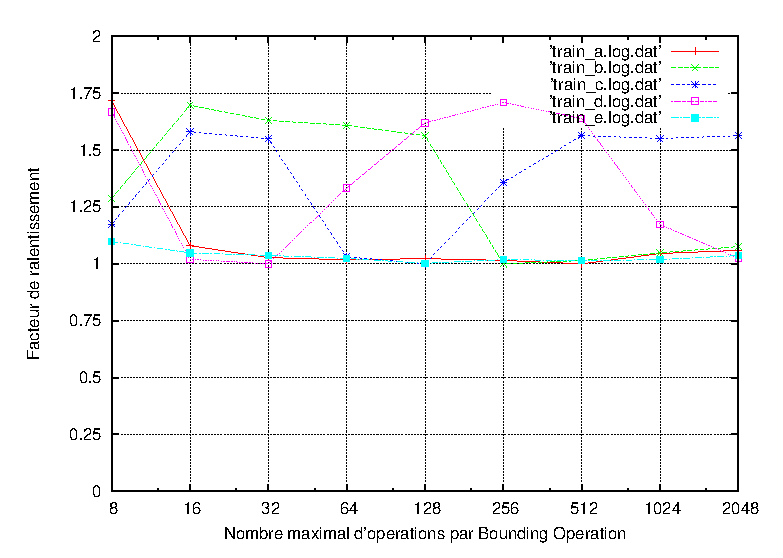
\includegraphics[width=\textwidth]{images/depthgraphd1.eps} 
					\caption{\label{fig:depthgraphd1}Performances de la troisième heuristique normalisées par leur meilleur temps}
				\end{figure}
				Les résultats sont résumés dans le tableau~\ref{boxdepth1}, page~\pageref{boxdepth1}, et repris sous forme normalisée par leur
				meilleur résultat au graphe~\ref{fig:depthgraphd1}, page~\pageref{fig:depthgraphd1}. 

				On constate que les différences de structure des dessins crée une grande variation dans les performances en fonction de
				la taille des \BO internes, ainsi que l'absence d'un optimum commun, prouvant la nécessité d'une heuristique plus complexe
				pour déterminer le moment optimum de fermeture des \BO internes. 

				On constate également que les performances n'atteignent pas les systèmes à un seul niveau pour les Dessins \emph{A,B,E}.
				Cela s'explique par le fait que ce dessins artificiels ne présentent pas des traits suffisamment longs et complexes pour 
				qu'une sous-séparation de ceux-ci soit bénéfique. 

				Par contre, si l'on observe quelque gains pour les dessins \emph{A} et \emph{B}, ceux-ci sont peu importants. Une raison possible
				est le fait que pour les traits plus petits la \BO interne est redondante. 
				
			\subsection{Conclusion}
				Le analyses de performances montrent que les \BO améliorent de manière substantielle les performances du framework pour la peinture.
				Cependant des améliorations restent possibles, comme une heuristique de clôture plus intelligente, qui permettrait des niveaux de 
				\BO supplémentaires qui englobent les états. 

				Enfin les tests se sont concentrés sur le temps de rendu moyen d'une opération, il pourrait être intéressant de tenter de réduire
				la variance des temps de rendu afin d'augmenter la fluidité lors d'édition interactive. 

%			\subsubsection{\emph{BOH} 2}
%				Cette troisième heuristique utilise également un \emph{BOH} à deux niveaux.
%
%				\begin{table*}
%					\tiny
%					\label{boxdepthr1}
%					\begin{tabular*}{\textwidth}{@{\extracolsep{\fill}} | c || c | c | c | c | c | c | c | c | }
%						\hline
%						Dessin & \multicolumn{8}{c|}{Temps de calcul (sec)} \\
%						\hline
%						\BO Internes 	& \multicolumn{4}{c|}{32}					&  \multicolumn{4}{c|}{64}	\\					
%						\hline
%						\BO Externes	& 4		&  8		&  16		&  32		&  4		&  8		&  16		&  32		       \\
%						\hline
%						A		& 45.88		&  37.45	&  34.88	&  33.09	&  37.64	&  33.91	&  32.77	&  33.04	       \\
%						B 		& 100.87	&  47.39	&  43.65	&  43.07	&  49.19	&  43.15	&  42.85	&  41.30	       \\
%						C 		& 127.49	&  137.28	&  142.36	&  136.36	&  103.51	&  108.55	&  140.65	&  140.19		\\
%						D		& 193.25	&  153.72	&  142.94	&  140.80	&  156.07	&  145.47	&  139.30	&  134.22		\\
%						E		& 19.08		&  17.22	&  17.02	&  16.51	&  17.87	&  16.68	&  14.64	&  11.18	       \\
%						\hline
%						\BO Internes 	&  \multicolumn{4}{c|}{128}					& \multicolumn{4}{c|}{256}   \\
%						\hline
%						\BO Externes	&  4 		&  8		&  16		&  32		&  4		&  8		& 16		&  32		\\
%						\hline
%						A		&  35.29	&  33.64	&  50.20	&  54.35	&  53.44	&  54.52	&  57.16	&  55.31	\\
%						B 		&  43.39	&  50.90	&  63.60	&  63.78	&  65.60	&  66.61	&  46.07	&  42.05	\\
%						C 		&  142.59	&  136.45	&  138.14	&  138.23	&  139.82	&  97.75	&  88.15	&  138.16	\\
%						D		&  139.39	&  141.59	&  91.14	&  88.86	&  137.26	&  137.37	&  137.34	&  137.08	\\
%						E		&  12.81	&  11.17	&  10.95	&  10.66	&  11.02	&  11.07	&  10.75	&  10.56	\\
%						\hline
%					\end{tabular*}
%				\end{table*}
%				\begin{figure}[h]
%					\centering
%					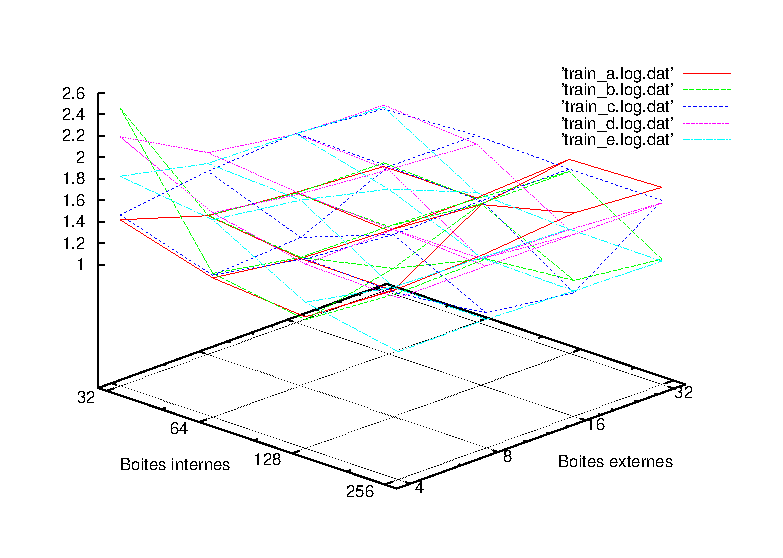
\includegraphics[width=\textwidth]{images/depthgraphr1.eps} 
%					\label{fig:depthgraphr1}
%				\end{figure}




